%%%%%%%%%%%%%%%%%%%%%%%%%%%%%%%%%%%%%%%%%
% Structured General Purpose Assignment
% LaTeX Template
%
% This template has been downloaded from:
% http://www.latextemplates.com
%
% Original author:
% Ted Pavlic (http://www.tedpavlic.com)
%
% Note:
% The \lipsum[#] commands throughout this template generate dummy text
% to fill the template out. These commands should all be removed when 
% writing assignment content.
%
%%%%%%%%%%%%%%%%%%%%%%%%%%%%%%%%%%%%%%%%%

%----------------------------------------------------------------------------------------
%	PACKAGES AND OTHER DOCUMENT CONFIGURATIONS
%----------------------------------------------------------------------------------------

\documentclass{article}

\usepackage[T1]{fontenc}
\usepackage[utf8]{inputenc}
\usepackage[francais]{babel}
\usepackage{fancyhdr} % Required for custom headers
\usepackage{lastpage} % Required to determine the last page for the footer
\usepackage{extramarks} % Required for headers and footers
\usepackage{graphicx} % Required to insert images
\usepackage{lipsum} % Used for inserting dummy 'Lorem ipsum' text into the template
\usepackage{amsmath,amsfonts,amssymb}


% Margins
\topmargin=-0.45in
\evensidemargin=0in
\oddsidemargin=0in
\textwidth=6.5in
\textheight=9.0in
\headsep=0.25in 

\linespread{1.1} % Line spacing

% Set up the header and footer
\pagestyle{fancy}
\lhead{\hmwkAuthorName} % Top left header
\chead{\hmwkClass: \hmwkTitle} % Top center header
\rhead{\firstxmark} % Top right header
\lfoot{\lastxmark} % Bottom left footer
\cfoot{} % Bottom center footer
\rfoot{Page\ \thepage\ de\ \pageref{LastPage}} % Bottom right footer
\renewcommand\headrulewidth{0.4pt} % Size of the header rule
\renewcommand\footrulewidth{0.4pt} % Size of the footer rule

\setlength\parindent{0pt} % Removes all indentation from paragraphs

%----------------------------------------------------------------------------------------
%	DOCUMENT STRUCTURE COMMANDS
%	Skip this unless you know what you're doing
%----------------------------------------------------------------------------------------

% Header and footer for when a page split occurs within a problem environment
\newcommand{\enterProblemHeader}[1]{
\nobreak\extramarks{#1}{#1 continue sur la page suivante\ldots}\nobreak
\nobreak\extramarks{#1 (continued)}{\textit{#1} continue sur la page suivante\ldots}\nobreak
}

% Header and footer for when a page split occurs between problem environments
\newcommand{\exitProblemHeader}[1]{
\nobreak\extramarks{#1 (continued)}{#1 continue sur la page suivante\ldots}\nobreak
\nobreak\extramarks{#1}{}\nobreak
}

\setcounter{secnumdepth}{0} % Removes default section numbers
\newcounter{homeworkProblemCounter} % Creates a counter to keep track of the number of problems

\newcommand{\homeworkProblemName}{}
\newenvironment{homeworkProblem}[1][Question \arabic{homeworkProblemCounter}]{ % Makes a new environment called homeworkProblem which takes 1 argument (custom name) but the default is "Problem #"
\stepcounter{homeworkProblemCounter} % Increase counter for number of problems
\renewcommand{\homeworkProblemName}{#1} % Assign \homeworkProblemName the name of the problem
\section{\homeworkProblemName} % Make a section in the document with the custom problem count
\enterProblemHeader{\homeworkProblemName} % Header and footer within the environment
}{
\exitProblemHeader{\homeworkProblemName} % Header and footer after the environment
}

\newcommand{\problemAnswer}[1]{ % Defines the problem answer command with the content as the only argument
\noindent\framebox[\columnwidth][c]{\begin{minipage}{0.98\columnwidth}#1\end{minipage}} % Makes the box around the problem answer and puts the content inside
}

\newcommand{\homeworkSectionName}{}
\newenvironment{homeworkSection}[1]{ % New environment for sections within homework problems, takes 1 argument - the name of the section
\renewcommand{\homeworkSectionName}{#1} % Assign \homeworkSectionName to the name of the section from the environment argument
\subsection{\homeworkSectionName} % Make a subsection with the custom name of the subsection
\enterProblemHeader{\homeworkProblemName\ [\homeworkSectionName]} % Header and footer within the environment
}{
\enterProblemHeader{\homeworkProblemName} % Header and footer after the environment
}
   
%----------------------------------------------------------------------------------------
%	NAME AND CLASS SECTION
%----------------------------------------------------------------------------------------

\newcommand{\hmwkTitle}{Rapport laboratoire 1} % Assignment title
\newcommand{\hmwkDueDate}{Mardi,\ 19\ Janvier\ 2016} % Due date
\newcommand{\hmwkClass}{INF-6422} % Course/class
\newcommand{\hmwkClassTime}{} % Class/lecture time
\newcommand{\hmwkClassInstructor}{Francois Labrèche} % Teacher/lecturer
\newcommand{\hmwkAuthorName}{Thomas Luinaud, Paul Berthier} % Your name

%----------------------------------------------------------------------------------------
%	TITLE PAGE
%----------------------------------------------------------------------------------------

\title{
\textmd{\textbf{\hmwkClass:\ \hmwkTitle}}\\
\normalsize\vspace{0.1in}\small{Rendu\ le\ \hmwkDueDate}\\
\vspace{0.1in}\large{à \textit{\hmwkClassInstructor\ \hmwkClassTime}}\\
\vspace{1in}

\includegraphics[width=200pt]{pictures/logo-poly.png}
\vspace{2in}
}

\author{\textbf{\hmwkAuthorName}}
\date{} % Insert date here if you want it to appear below your name

%----------------------------------------------------------------------------------------

\begin{document}

	\maketitle
	
	%----------------------------------------------------------------------------------------
	%	TABLE OF CONTENTS
	%----------------------------------------------------------------------------------------
	
	%\setcounter{tocdepth}{1} % Uncomment this line if you don't want subsections listed in the ToC
	
	\newpage
	\tableofcontents
	\newpage
	
	\begin{homeworkProblem}[Mise en contexte]
	
	
		\begin{homeworkSection}{1.1}
		
			L’épidémiologie pourrait être définie comme l’étude des rapports existant entre les
			maladies ou tout autre phénomène biologique, et divers facteurs susceptibles d’exercer
			une influence sur leur fréquence, distribution et évolution. Entre d’autres mots,
			l’épidémiologie s’intéresse aux facteurs qui influencent la santé des populations. Plus
			particulièrement, l’épidémiologie s’intéresse, entre autre, à étudier la dynamique de
			propagation des maladies infectieuses afin d’établir des stratégies de prévention et
			d’intervention permettant de diminuer l’impact sur la santé publique. À cet effet, la
			modélisation mathématique s’est révélée particulièrement intéressante afin de simuler des
			scénarios épidémiologiques, d’évaluer les risques associés et de quantifier l’efficacité et
			l’impact de différentes méthodes d’intervention et de prévention. Plusieurs approches
			peuvent être retenues, telles que les simulations numériques, les modèles déterministes ou
			encore les modèles stochastiques. Chaque approche présente des avantages et des
			inconvénients. Il convient donc de choisir la méthode la plus appropriée en fonction des
			questions de recherche auxquelles vous souhaitez répondre.
			
		\end{homeworkSection}
		
		\begin{homeworkSection}{1.2}
		
			Appliquée à la sécurité informatique, l’épidémiologie pourrait être vue comme l’étude
			des différents facteurs qui influencent la fréquence, la distribution et l’évolution des
			logiciels malveillants. Plus particulièrement, l’approche épidémiologique a inspiré de
			nombreux travaux de recherche portant sur l’étude de la propagation des logiciels
			malveillants. Le présent laboratoire vous permettra de vous familiariser avec certaines
			approches mathématiques fréquemment utilisées afin de modéliser la propagation de
			logiciels malveillants au sein d’un réseau.
		
		\end{homeworkSection}
	
	\end{homeworkProblem}
	
	
%----------------------------------------------------------------------------------------
%	PROBLEM 1
%----------------------------------------------------------------------------------------

% To have just one problem per page, simply put a \clearpage after each problem

\begin{homeworkProblem}
Une approche très répandue dans l’étude de la propagation des logiciels malveillants
consiste à développer un modèle déterministe basé sur les concepts de compartiments et
de règles [2]. Les compartiments servent à diviser la population étudiée en différentes
classes et les règles à définir les conditions de transition entre chacune des classes.
\begin{homeworkSection}{1.1}
En vous basant sur l’article « Optimising Networks Against Malware » [3], quel
modèle comportemental (SI, SIS, SIR) s’appliquerait et pourquoi? Justifiez votre réponse
en expliquant quel modèle s’applique et pourquoi les autres modèles ne s’appliquent pas.

\problemAnswer{ % Answer
Dans un premier temps
}
\end{homeworkSection}
\end{homeworkProblem}

% %----------------------------------------------------------------------------------------
% %	PROBLEM 2
% %----------------------------------------------------------------------------------------

\begin{homeworkProblem}
% Question
Lors de la question précédente, vous avez développé un modèle théorique basé sur un
système d’équations différentielles. Heureusement, il existe une solution analytique à ce
système afin de représenter le nombre de machines infectées en fonction du temps :
\begin{equation}
I(t)=\frac{I_0 N}{(N-I_0)e^{-\lambda t}+I_0}
\label{moneq}
\end{equation}

% %--------------------------------------------

% \begin{homeworkSection}{(a)} % Section within problem
% \lipsum[4]\vspace{10pt} % Question

% %\problemAnswer{ % Answer
% %\lipsum[5]
% %}
%\end{homeworkSection}

% %--------------------------------------------

% \begin{homeworkSection}{(b)} % Section within problem
% %\problemAnswer{ % Answer
% %\lipsum[6]
% %}
% \end{homeworkSection}

% %--------------------------------------------
\end{homeworkProblem}
	% %----------------------------------------------------------------------------------------
% %	PROBLEM 4
% %----------------------------------------------------------------------------------------


\begin{homeworkProblem}[Modèle stochastique]
	
	Dans l’article « Optimising networks Against Malware », l’auteur utilise un modèle
	stochastique basé sur les chaînes de Markov afin de modéliser la propagation d’un vers
	dans un réseau .
	
	\begin{homeworkSection}{4.1}
	
		Expliquez les caractéristiques d’un modèle stochastique et pourquoi ce type de
		modèle s’applique dans le contexte de l’article. Est-ce qu’une approche déterministe
		aurait été préférable? \\
		
		\problemAnswer{
		
		Un modèle stochastique repose sur des variables aléatoires représentant l'évolution possible d'un système au cours du temps. Ce type de modèle s'applique très bien dans le contexte de l'article car on modélise l'évolution de l'infection d'un système de machines au cours du temps, chaque ensemble de machines infectées étant représenté par un état, avec une certaine probabilité \textit{p} de passer à un autre état au temps \textit{t+1} (chaines de Markov).\\
		Une approche déterministe n'aurait pas été réalisable, car les résultats de l'expérience ne sont pas fixes, et donc pas reproductibles. En effet, l'évolution de l'infection dépend de la rapidité à laquelle la première machine infectée réussit à atteindre le \textit{gateway} afin d'atteindre l'autre sous-réseau. Cela se vérifie sur la \ref{ExpG4}, où l'on voit que l'intervalle de confiance de l'expérience est très large.
		
		}
		
		\begin{figure}[h]
			\caption{\label{ExpG4} Expérience avec G=4}
			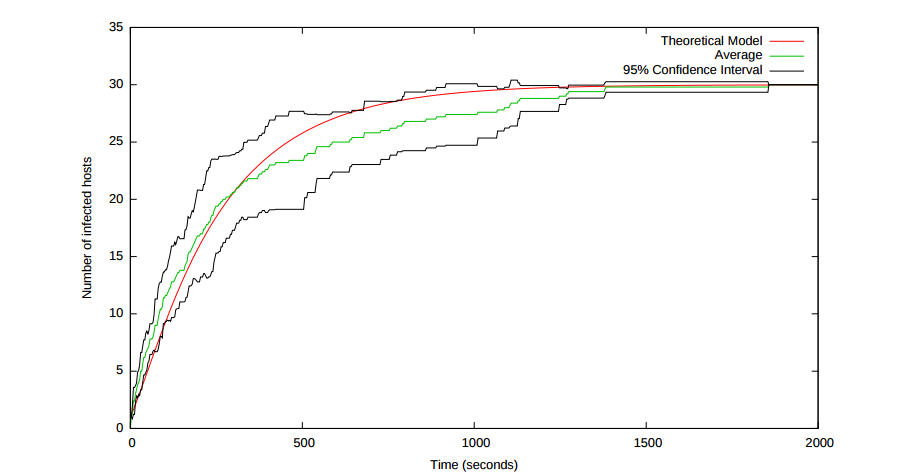
\includegraphics[width=\textwidth]{pictures/results-G=4.png}
		\end{figure}
		
	\end{homeworkSection}

\end{homeworkProblem}

% %----------------------------------------------------------------------------------------
% %	PROBLEM 5
% %----------------------------------------------------------------------------------------

\begin{homeworkProblem}[Performance et optimisation]

	Toujours dans l’article « Optimising networks Against Malware », l’auteur étudie
	l’effet de la topologie du réseau sur la vitesse de propagation d’un vers informatique.\\
	
	\begin{homeworkSection}{5.1}
	
		Appliquez le concept du double-tétraèdre étudié en classe à l’article. Situez votre
		double-tétraèdre dans un contexte d’optimisation, toujours en vous référant à l’article.
		Expliquez quels sont les aspects de votre double-tétraèdre qui sont fixes, et ceux qui sont
		modifiés.\\
		
		\problemAnswer{
			Le double-tétraèdre étudié en classe regroupe les propriétés suivantes :
			\begin{itemize}
				\item L'\textbf{environnement}, commun à l'attaquant et au défenseur
				\item Des \textbf{critères de performance}, propres à l'attaquant et au défenseur
				\item Les \textbf{caractéristiques} de l'attaque et de la défense\\
			\end{itemize}
			
			Les caractéristiques suivantes sont fixées:
			\begin{itemize}
				\item \textbf{Les caractéristiques de l'attaque} : On utilise le \textit{Malware Emulation Framework}, qui produit un ver qui se reproduit en scannant les ip des machines voisines.
				\item \textbf{Les caractéristiques de la défense} : Il n'y en a pas. Dés que l'attaquant scanne l'ip d'une machine, celle-ci est infectée.
				\item \textbf{Le critère de performance de l'attaque} : La vitesse de propagation du virus sur le réseau.
				\item \textbf{Le critère de performance de la défense} : C'est également la vitesse de propagation du virus sur le réseau, mais dans le sens inverse (on souhaite que le virus se propage le plus lentement possible ...)\\
			\end{itemize}
			
			Le seul paramètre variable est l'environnement : on va faire varier la topologie du réseau en jouant sur le nombre de \textit{gateway} interconnectant les différents sous-réseaux.\\
			
			On est donc en présence d'un problème d'optimisation du critère de performance, c'est à dire la vitesse de propagation du ver sur le réseau (qui doit être la plus lente possible du point de vue du défenseur), la variable étant le nombre de \textit{gateway}.
				
		}
		
	\end{homeworkSection}
	
	\begin{homeworkSection}{5.2}
	
		Quels autres aspects/méthodes (autres que la topologie du réseau) pourraient être
		étudiés dans le cadre d’un problème d’optimisation où l’objectif est de limiter la vitesse
		de propagation d’un logiciel malveillant dans un réseau? Donnez au minimum deux
		exemples.\\

		\problemAnswer{
		
			Les autre méthodes suivantes pourraient être étudiées afin de limiter la propagation d'un logiciel malveillant dans le réseau:
			
			\begin{itemize}
				\item L'utilisation d'un \textit{firewall}, filtrant l'utilisation de certains ports, traditionnellement utilisés pour transmettre des virus (telnet, ...)
				\item Le blocage de certains paquets ICMP (comme le \textit{ECHO} utilisé par la commande \textit{Ping}) afin d'empêcher l'attaquant de scanner les ports ouverts d'une machine.
				\item L'utilisation d'un antivirus ayant une base de donnée des signatures des virus connus, ou étant capable de reconnaître les comportements suspects des virus (ouverture de connexion sur des ports peu usités, ...)
				\item Demander à l'utilisateur une confirmation avant l'installation de tout programme en provenance du réseau.
			\end{itemize}
			
		
		}
	
	\end{homeworkSection}
	
	\begin{homeworkSection}{5.3}
		
		Il a été démontré qu’une plus grande biodiversité au sein d’un écosystème permettait
		de ralentir la propagation des virus ou des bactéries dangereuses. Comment pourriez-vous
		appliquer le concept de diversité au sein d’un réseau informatique? Quelle(s) forme(s)
		prendrait cette diversité? \\
		
		\problemAnswer{

		
		}
	
	\end{homeworkSection}


\end{homeworkProblem}


\end{document}
